% !TeX spellcheck = hu_HU
% !TeX encoding = UTF-8
% !TeX program = xelatex
% TODO Change language to en_GB (recommended) or en_US for English documents
\documentclass[11pt,a4paper,oneside]{report}             % Single-side
%\documentclass[11pt,a4paper,twoside,openright]{report}  % Duplex

% thanks to http://tex.stackexchange.com/a/47579/71109
\usepackage{ifxetex}
\usepackage{ifluatex}
\newif\ifxetexorluatex % a new conditional starts as false
\ifnum 0\ifxetex 1\fi\ifluatex 1\fi>0
   \xetexorluatextrue
\fi

\ifxetexorluatex
  \usepackage{fontspec}
\else
  \usepackage[T1]{fontenc}
  \usepackage[utf8]{inputenc}
  \usepackage[lighttt]{lmodern}
\fi

\usepackage[english,magyar]{babel} % Alapértelmezés szerint utoljára definiált nyelv lesz aktív, de később külön beállítjuk az aktív nyelvet.

%\usepackage{cmap}
\usepackage{amsfonts,amsmath,amssymb} % Mathematical symbols.
%\usepackage[ruled,boxed,resetcount,linesnumbered]{algorithm2e} % For pseudocodes. % beware: this is not compatible with LuaLaTeX, see http://tex.stackexchange.com/questions/34814/lualatex-and-algorithm2e
\usepackage{booktabs} % For publication quality tables for LaTeX
\usepackage{graphicx}

%\usepackage{fancyhdr}
%\usepackage{lastpage}

\usepackage{anysize}
%\usepackage{sectsty}
\usepackage{setspace} % For setting line spacing

\usepackage[unicode]{hyperref} % For hyperlinks in the generated document.
\usepackage{xcolor}
\usepackage{listings} % For source code snippets.

\usepackage[amsmath,thmmarks]{ntheorem} % Theorem-like environments.

\usepackage[hang]{caption}

\singlespacing

\newcommand{\selecthungarian}{
	\selectlanguage{magyar}
	\setlength{\parindent}{2em}
	\setlength{\parskip}{0em}
	\frenchspacing
}

\newcommand{\selectenglish}{
	\selectlanguage{english}
	\setlength{\parindent}{0em}
	\setlength{\parskip}{0.5em}
	\nonfrenchspacing
	\renewcommand{\figureautorefname}{Figure}
	\renewcommand{\tableautorefname}{Table}
	\renewcommand{\partautorefname}{Part}
	\renewcommand{\chapterautorefname}{Chapter}
	\renewcommand{\sectionautorefname}{Section}
	\renewcommand{\subsectionautorefname}{Section}
	\renewcommand{\subsubsectionautorefname}{Section}
}

\usepackage[numbers]{natbib}
\usepackage{xspace}


\usepackage{xcolor}

\definecolor{codegreen}{rgb}{0,0.6,0}
\definecolor{codegray}{rgb}{0.5,0.5,0.5}
\definecolor{codepurple}{rgb}{0.58,0,0.82}
\definecolor{backcolour}{rgb}{0.95,0.95,0.92}


\lstdefinestyle{mystyle}{
	backgroundcolor=\color{backcolour},   
	commentstyle=\color{codegreen},
	keywordstyle=\color{magenta},
	numberstyle=\tiny\color{codegray},
	stringstyle=\color{codepurple},
	basicstyle=\ttfamily\footnotesize,
	breakatwhitespace=false,         
	breaklines=true,                 
	captionpos=b,                    
	keepspaces=true,                 
	numbers=left,                    
	numbersep=5pt,                  
	showspaces=false,                
	showstringspaces=false,
	showtabs=false,                  
	tabsize=2
}

\lstdefinelanguage{docker-compose-proxy}{
	keywords={version, volumes, services, proxy, restart, build, ports},
	keywordstyle=\color{blue}\bfseries,
	%keywords=[2]{image, environment, ports, container_name, ports, links, build},
	keywordstyle=[2]\color{olive}\bfseries,
	identifierstyle=\color{black},
	sensitive=false,
	comment=[l]{\#},
	commentstyle=\color{purple}\ttfamily,
	stringstyle=\color{red}\ttfamily,
	morestring=[b]',
	morestring=[b]"
}


%---


%TODO Set the main variables
\newcommand{\vikszerzoVezeteknev}{Orova}
\newcommand{\vikszerzoKeresztnev}{Márton}

\newcommand{\vikkonzulensAMegszolitas}{dr.~}
\newcommand{\vikkonzulensAVezeteknev}{Szatmári}
\newcommand{\vikkonzulensAKeresztnev}{Zoltán}

\newcommand{\vikkonzulensBMegszolitas}{}
\newcommand{\vikkonzulensBVezeteknev}{Simon}
\newcommand{\vikkonzulensBKeresztnev}{Attila}

\newcommand{\vikkonzulensCMegszolitas}{}
\newcommand{\vikkonzulensCVezeteknev}{}
\newcommand{\vikkonzulensCKeresztnev}{}

\newcommand{\vikcim}{Integration of standard datasources with interactive data visualization solutions} % Cím
\newcommand{\viktanszek}{\bmemit} % Tanszék
\newcommand{\vikdoktipus}{\bsc} % Dokumentum típusa (\bsc vagy \msc)
\newcommand{\vikmunkatipusat}{szakdolgozatot} % a "hallgató nyilatkozat" részhez: szakdolgozatot vagy diplomatervet

%--------------------------------------------------------------------------------------
% TDK-specifikus változók
%--------------------------------------------------------------------------------------
\newcommand{\tdkszerzoB}{Második Szerző} % Második szerző neve; hagyd üresen, ha egyedül írtad a TDK-t.
\newcommand{\tdkev}{2014} % A dolgozat írásának éve (pl. "2014") (Ez OTDK-nál eltérhet az aktuális évtől.)

% További adatok az OTDK címlaphoz (BME-s TDK-hoz nem kell kitölteni)
\newcommand{\tdkevfolyamA}{IV} % Első szerző évfolyama, római számmal (pl. IV).
\newcommand{\tdkevfolyamB}{III} % Második szerző évfolyama, római számmal (pl. III).
\newcommand{\tdkkonzulensbeosztasA}{egyetemi tanár} % Első konzulens beosztása (pl. egyetemi docens)
\newcommand{\tdkkonzulensbeosztasB}{doktorandusz} % Második konzulens beosztása (pl. egyetemi docens)

\newcommand{\szerzoMeta}{\vikszerzoVezeteknev{} \vikszerzoKeresztnev} % egy szerző esetén
%\newcommand{\szerzoMeta}{\vikszerzoVezeteknev{} \vikszerzoKeresztnev, \tdkszerzoB} % két szerző esetén

%TODO Language configuration -- choose one
% Beállítások magyar nyelvű dolgozathoz
%%--------------------------------------------------------------------------------------
% Elnevezések
%--------------------------------------------------------------------------------------
\newcommand{\bme}{Budapesti Műszaki és Gazdaságtudományi Egyetem}
\newcommand{\vik}{Villamosmérnöki és Informatikai Kar}

\newcommand{\bmemit}{Méréstechnika és Információs Rendszerek Tanszék}

\newcommand{\keszitette}{Készítette}
\newcommand{\konzulens}{Konzulens}

\newcommand{\bsc}{Szakdolgozat}
\newcommand{\msc}{Diplomaterv}
\newcommand{\tdk}{TDK dolgozat}
\newcommand{\bsconlab}{BSc Önálló laboratórium}
\newcommand{\msconlabi}{MSc Önálló laboratórium 1.}
\newcommand{\msconlabii}{MSc Önálló laboratórium 2.}

\newcommand{\pelda}{Példa}
\newcommand{\definicio}{Definíció}
\newcommand{\tetel}{Tétel}

\newcommand{\bevezetes}{Bevezetés}
\newcommand{\koszonetnyilvanitas}{Köszönetnyilvánítás}
\newcommand{\fuggelek}{Függelék}

% Opcionálisan átnevezhető címek
%\addto\captionsmagyar{%
%\renewcommand{\listfigurename}{Saját ábrajegyzék cím}
%\renewcommand{\listtablename}{Saját táblázatjegyzék cím}
%\renewcommand{\bibname}{Saját irodalomjegyzék név}
%}

\newcommand{\szerzo}{\vikszerzoVezeteknev{} \vikszerzoKeresztnev}
\newcommand{\vikkonzulensA}{\vikkonzulensAMegszolitas\vikkonzulensAVezeteknev{} \vikkonzulensAKeresztnev}
\newcommand{\vikkonzulensB}{\vikkonzulensBMegszolitas\vikkonzulensBVezeteknev{} \vikkonzulensBKeresztnev}
\newcommand{\vikkonzulensC}{\vikkonzulensCMegszolitas\vikkonzulensCVezeteknev{} \vikkonzulensCKeresztnev}

\newcommand{\selectthesislanguage}{\selecthungarian}

\bibliographystyle{huplain}

\def\lstlistingname{lista}

\newcommand{\appendixnumber}{6}  % a fofejezet-szamlalo az angol ABC 6. betuje (F) lesz

% Settings for English documents
%--------------------------------------------------------------------------------------
% Elnevezések
%--------------------------------------------------------------------------------------
\newcommand{\bme}{Budapest University of Technology and Economics}
\newcommand{\vik}{Faculty of Electrical Engineering and Informatics}

\newcommand{\bmemit}{Department of Measurement and Information Systems}

\newcommand{\keszitette}{Author}
\newcommand{\konzulens}{Advisor}

\newcommand{\bsc}{Bachelor's Thesis}
\newcommand{\msc}{Master's Thesis}
\newcommand{\tdk}{Scientific Students' Association Report}
\newcommand{\bsconlab}{BSc Project Laboratory}
\newcommand{\msconlabi}{MSc Project Laboratory 1}
\newcommand{\msconlabii}{MSc Project Laboratory 2}

\newcommand{\pelda}{Example}
\newcommand{\definicio}{Definition}
\newcommand{\tetel}{Theorem}

\newcommand{\bevezetes}{Introduction}
\newcommand{\koszonetnyilvanitas}{Acknowledgements}
\newcommand{\fuggelek}{Appendix}

% Optional custom titles
%\addto\captionsenglish{%
%\renewcommand*{\listfigurename}{Your list of figures title}
%\renewcommand*{\listtablename}{Your list of tables title}
%\renewcommand*{\bibname}{Your bibliography title}
%}

\newcommand{\szerzo}{\vikszerzoKeresztnev{} \vikszerzoVezeteknev}
\newcommand{\vikkonzulensA}{\vikkonzulensAMegszolitas\vikkonzulensAKeresztnev{} \vikkonzulensAVezeteknev}
\newcommand{\vikkonzulensB}{\vikkonzulensBMegszolitas\vikkonzulensBKeresztnev{} \vikkonzulensBVezeteknev}
\newcommand{\vikkonzulensC}{\vikkonzulensCMegszolitas\vikkonzulensCKeresztnev{} \vikkonzulensCVezeteknev}

\newcommand{\selectthesislanguage}{\selectenglish}

\bibliographystyle{plainnat}

\newcommand{\ie}{i.e.\@\xspace}
\newcommand{\Ie}{I.e.\@\xspace}
\newcommand{\eg}{e.g.\@\xspace}
\newcommand{\Eg}{E.g.\@\xspace}
\newcommand{\etal}{et al.\@\xspace}
\newcommand{\etc}{etc.\@\xspace}
\newcommand{\vs}{vs.\@\xspace}
\newcommand{\viz}{viz.\@\xspace} % videlicet
\newcommand{\cf}{cf.\@\xspace} % confer
\newcommand{\Cf}{Cf.\@\xspace}
\newcommand{\wrt}{w.r.t.\@\xspace} % with respect to
\newcommand{\approximately}{approx.\@\xspace}

\newcommand{\appendixnumber}{1}  % a fofejezet-szamlalo az angol ABC 1. betuje (A) lesz


%--------------------------------------------------------------------------------------
% Page layout setup
%--------------------------------------------------------------------------------------
% we need to redefine the pagestyle plain
% another possibility is to use the body of this command without \fancypagestyle
% and use \pagestyle{fancy} but in that case the special pages
% (like the ToC, the References, and the Chapter pages)remain in plane style

\pagestyle{plain}
\marginsize{35mm}{25mm}{15mm}{15mm}

\setcounter{tocdepth}{3}
%\sectionfont{\large\upshape\bfseries}
\setcounter{secnumdepth}{3}

\sloppy % Margón túllógó sorok tiltása.
\widowpenalty=10000 \clubpenalty=10000 %A fattyú- és árvasorok elkerülése
\def\hyph{-\penalty0\hskip0pt\relax} % Kötőjeles szavak elválasztásának engedélyezése


%--------------------------------------------------------------------------------------
% Setup hyperref package
%--------------------------------------------------------------------------------------
\hypersetup{
    % bookmarks=true,            % show bookmarks bar?
    unicode=true,              % non-Latin characters in Acrobat's bookmarks
    pdftitle={\vikcim},        % title
    pdfauthor={\szerzoMeta},    % author
    pdfsubject={\vikdoktipus}, % subject of the document
    pdfcreator={\szerzoMeta},   % creator of the document
    pdfproducer={},    % producer of the document
    pdfkeywords={},    % list of keywords (separate then by comma)
    pdfnewwindow=true,         % links in new window
    colorlinks=true,           % false: boxed links; true: colored links
    linkcolor=black,           % color of internal links
    citecolor=black,           % color of links to bibliography
    filecolor=black,           % color of file links
    urlcolor=black             % color of external links
}


%--------------------------------------------------------------------------------------
% Set up listings
%--------------------------------------------------------------------------------------
\definecolor{lightgray}{rgb}{0.95,0.95,0.95}
\lstset{
	basicstyle=\scriptsize\ttfamily, % print whole listing small
	keywordstyle=\color{black}\bfseries, % bold black keywords
	identifierstyle=, % nothing happens
	% default behavior: comments in italic, to change use
	% commentstyle=\color{green}, % for e.g. green comments
	stringstyle=\scriptsize,
	showstringspaces=false, % no special string spaces
	aboveskip=3pt,
	belowskip=3pt,
	backgroundcolor=\color{lightgray},
	columns=flexible,
	keepspaces=true,
	escapeinside={(*@}{@*)},
	captionpos=b,
	breaklines=true,
	frame=single,
	float=!ht,
	tabsize=2,
	literate=*
		{á}{{\'a}}1	{é}{{\'e}}1	{í}{{\'i}}1	{ó}{{\'o}}1	{ö}{{\"o}}1	{ő}{{\H{o}}}1	{ú}{{\'u}}1	{ü}{{\"u}}1	{ű}{{\H{u}}}1
		{Á}{{\'A}}1	{É}{{\'E}}1	{Í}{{\'I}}1	{Ó}{{\'O}}1	{Ö}{{\"O}}1	{Ő}{{\H{O}}}1	{Ú}{{\'U}}1	{Ü}{{\"U}}1	{Ű}{{\H{U}}}1
}


%--------------------------------------------------------------------------------------
% Set up theorem-like environments
%--------------------------------------------------------------------------------------
% Using ntheorem package -- see http://www.math.washington.edu/tex-archive/macros/latex/contrib/ntheorem/ntheorem.pdf

\theoremstyle{plain}
\theoremseparator{.}
\newtheorem{example}{\pelda}

\theoremseparator{.}
%\theoremprework{\bigskip\hrule\medskip}
%\theorempostwork{\hrule\bigskip}
\theorembodyfont{\upshape}
\theoremsymbol{{\large \ensuremath{\centerdot}}}
\newtheorem{definition}{\definicio}

\theoremseparator{.}
%\theoremprework{\bigskip\hrule\medskip}
%\theorempostwork{\hrule\bigskip}
\newtheorem{theorem}{\tetel}


%--------------------------------------------------------------------------------------
% Some new commands and declarations
%--------------------------------------------------------------------------------------
\newcommand{\code}[1]{{\upshape\ttfamily\scriptsize\indent #1}}
\newcommand{\doi}[1]{DOI: \href{http://dx.doi.org/\detokenize{#1}}{\raggedright{\texttt{\detokenize{#1}}}}} % A hivatkozások közt így könnyebb DOI-t megadni.

\DeclareMathOperator*{\argmax}{arg\,max}
%\DeclareMathOperator*[1]{\floor}{arg\,max}
\DeclareMathOperator{\sign}{sgn}
\DeclareMathOperator{\rot}{rot}


%--------------------------------------------------------------------------------------
% Setup captions
%--------------------------------------------------------------------------------------
\captionsetup[figure]{
	width=.75\textwidth,
	aboveskip=10pt}

\renewcommand{\captionlabelfont}{\bf}
%\renewcommand{\captionfont}{\footnotesize\it}

%--------------------------------------------------------------------------------------
% Hyphenation exceptions
%--------------------------------------------------------------------------------------
\hyphenation{Shakes-peare Mar-seilles ár-víz-tű-rő tü-kör-fú-ró-gép}


\author{\vikszerzo}
\title{\viktitle}

%\renewcommand{\baselinestretch}{1.5}



%--------------------------------------------------------------------------------------
% Table of contents and the main text
%--------------------------------------------------------------------------------------
\begin{document}
\onehalfspacing
\lstset{style=mystyle}

\pagenumbering{gobble}

%TODO These includes define guidelines -- remove these
%~~~~~~~~~~~~~~~~~~~~~~~~~~~~~~~~~~~~~~~~~~~~~~~~~~~~~~~~~~~~~~~~~~~~~~~~~~~~~~~~~~~~~~
%\selecthungarian
%--------------------------------------------------------------------------------------
% Rovid formai es tartalmi tajekoztato
%--------------------------------------------------------------------------------------

\footnotesize
\begin{center}
\large
\textbf{\Large Általános információk, a diplomaterv szerkezete}\\
\end{center}

A diplomaterv szerkezete a BME Villamosmérnöki és Informatikai Karán:
\begin{enumerate}
\item	Diplomaterv feladatkiírás
\item	Címoldal
\item	Tartalomjegyzék
\item	A diplomatervező nyilatkozata az önálló munkáról és az elektronikus adatok kezeléséről
\item	Tartalmi összefoglaló magyarul és angolul
\item	Bevezetés: a feladat értelmezése, a tervezés célja, a feladat indokoltsága, a diplomaterv felépítésének rövid összefoglalása
\item	A feladatkiírás pontosítása és részletes elemzése
\item	Előzmények (irodalomkutatás, hasonló alkotások), az ezekből levonható következtetések
\item	A tervezés részletes leírása, a döntési lehetőségek értékelése és a választott megoldások indoklása
\item	A megtervezett műszaki alkotás értékelése, kritikai elemzése, továbbfejlesztési lehetőségek
\item	Esetleges köszönetnyilvánítások
\item	Részletes és pontos irodalomjegyzék
\item	Függelék(ek)
\end{enumerate}

Felhasználható a következő oldaltól kezdődő \LaTeX diplomatervsablon dokumentum tartalma. 

A diplomaterv szabványos méretű A4-es lapokra kerüljön. Az oldalak tükörmargóval készüljenek (mindenhol 2,5~cm, baloldalon 1~cm-es kötéssel). Az alapértelmezett betűkészlet a 12 pontos Times New Roman, másfeles sorközzel, de ettől kismértékben el lehet térni, ill. más betűtípus használata is megengedett.

Minden oldalon -- az első négy szerkezeti elem kivételével -- szerepelnie kell az oldalszámnak.

A fejezeteket decimális beosztással kell ellátni. Az ábrákat a megfelelő helyre be kell illeszteni, fejezetenként decimális számmal és kifejező címmel kell ellátni. A fejezeteket decimális aláosztással számozzuk, maximálisan 3 aláosztás mélységben (pl. 2.3.4.1.). Az ábrákat, táblázatokat és képleteket célszerű fejezetenként külön számozni (pl. 2.4. ábra, 4.2. táblázat vagy képletnél (3.2)). A fejezetcímeket igazítsuk balra, a normál szövegnél viszont használjunk sorkiegyenlítést. Az ábrákat, táblázatokat és a hozzájuk tartozó címet igazítsuk középre. A cím a jelölt rész alatt helyezkedjen el.

A képeket lehetőleg rajzoló programmal készítsék el, az egyenleteket egyenlet-szerkesztő segítségével írják le (A \LaTeX~ehhez kézenfekvő megoldásokat nyújt).

Az irodalomjegyzék szövegközi hivatkozása történhet sorszámozva (ez a preferált megoldás) vagy a Harvard-rendszerben (a szerző és az évszám megadásával). A teljes lista névsor szerinti sorrendben a szöveg végén szerepeljen (sorszámozott irodalmi hivatkozások esetén hivatkozási sorrendben). A szakirodalmi források címeit azonban mindig az eredeti nyelven kell megadni, esetleg zárójelben a fordítással. A listában szereplő valamennyi publikációra hivatkozni kell a szövegben (a \LaTeX-sablon a Bib\TeX~segítségével mindezt automatikusan kezeli). Minden publikáció a szerzők után a következő adatok szerepelnek: folyóirat cikkeknél a pontos cím, a folyóirat címe, évfolyam, szám, oldalszám tól-ig. A folyóiratok címét csak akkor rövidítsük, ha azok nagyon közismertek vagy nagyon hosszúak. Internetes hivatkozások megadásakor fontos, hogy az elérési út előtt megadjuk az oldal tulajdonosát és tartalmát (mivel a link egy idő után akár elérhetetlenné is válhat), valamint az elérés időpontját.

\vspace{5mm}
Fontos:
\begin{itemize}
	\item A szakdolgozatkészítő / diplomatervező nyilatkozata (a jelen sablonban szereplő szövegtartalommal) kötelező előírás, Karunkon ennek hiányában a szakdolgozat/diplomaterv nem bírálható és nem védhető!
	\item Mind a dolgozat, mind a melléklet maximálisan 15~MB méretű lehet!
\end{itemize}

\vspace{5mm}
\begin{center}
Jó munkát, sikeres szakdolgozatkészítést, ill. diplomatervezést kívánunk!
\end{center}

\normalsize
\selectthesislanguage

%%--------------------------------------------------------------------------------------
% Feladatkiiras (a tanszeken atveheto, kinyomtatott valtozat)
%--------------------------------------------------------------------------------------
\clearpage
\begin{center}
\large
\textbf{FELADATKIÍRÁS}\\
\end{center}

A feladatkiírást a tanszéki adminisztrációban lehet átvenni, és a leadott munkába eredeti, tanszéki pecséttel ellátott és a tanszékvezető által aláírt lapot kell belefűzni (ezen oldal \emph{helyett}, ez az oldal csak útmutatás). Az elektronikusan feltöltött dolgozatban már nem kell beleszerkeszteni ezt a feladatkiírást.


\selectthesislanguage

%TODO Titlepage -- choose one from below
%~~~~~~~~~~~~~~~~~~~~~~~~~~~~~~~~~~~~~~~~~~~~~~~~~~~~~~~~~~~~~~~~~~~~~~~~~~~~~~~~~~~~~~
\hypersetup{pageanchor=false}
%--------------------------------------------------------------------------------------
%	The title page
%--------------------------------------------------------------------------------------
\begin{titlepage}
\begin{center}

\includegraphics[width=60mm,keepaspectratio]{figures/bme_logo.pdf}\\
\vspace{0.3cm}
\textbf{\bme}\\
\textmd{\vik}\\
\textmd{\viktanszek}\\[5cm]

\vspace{0.4cm}
{\huge \bfseries \vikcim}\\[0.8cm]
\vspace{0.5cm}
\textsc{\Large \vikdoktipus}\\[4cm]

{
	\renewcommand{\arraystretch}{0.85}
	\begin{tabular}{cc}
	 \makebox[7cm]{\emph{\keszitette}} & \makebox[7cm]{\emph{\konzulens}} \\ \noalign{\smallskip}
	 \makebox[7cm]{\szerzo} & \makebox[7cm]{\vikkonzulensA} \\
	  & \makebox[7cm]{\vikkonzulensB} \\
	  & \makebox[7cm]{\vikkonzulensC} \\
	\end{tabular}
}

\vfill
{\large \today}
\end{center}
\end{titlepage}
\hypersetup{pageanchor=false}

		   % Szakdolgozat/Diplomaterv címlap
%%% TDK címlap
\begin{titlepage}
  \begin{center}  
  
\includegraphics[width=7cm]{./figures/bme_logo.pdf}
  \vspace{0.3cm}
  
  \bme \\
  \vik \\
  \viktanszek \\
  \vspace{5cm}
  
  \huge {\vikcim}
  \vspace{1.5cm}
  
  \large {\textbf{\tdk}}
  \vfill
    
  {\Large 
  	\keszitette: \\ \vspace{0.3cm}
  	\szerzo \\
	\tdkszerzoB \\
  	\vspace{1.5cm}
  	\konzulens: \\ \vspace{0.3cm}
  	\vikkonzulensA \\
  	\vikkonzulensB \\
  }
  
  \vspace{2cm}
  \large {\tdkev}
 \end{center}
\end{titlepage}
%% Címlap vége
	% TDK címlap
%%% OTDK külső címlap
\begin{titlepage}
  	$\;$ 
	\vspace{5cm}
	
	\begin{center}
	\Huge
	\textbf{TDK-dolgozat}\let\thefootnote\relax\footnote{A dolgozat bemutatását a XXXXXXXXX  ``Lorem ipsum dolor sit amet'' című program támogatta.}
	\end{center}
	
	\vspace{13cm}
	
	\Large
	\hspace{8cm} \szerzo
	
	\hspace{8cm} \tdkszerzoB
	
	\hspace{8cm} \tdkev.
\end{titlepage}

\newpage
\thispagestyle{empty}


%% OTDK belső címlap
\begin{titlepage}
  \begin{center}  
  
\includegraphics[width=7cm]{./figures/bme_logo.pdf}
  \vspace{0.3cm}
  
  \bme \\
  \vik \\
  \viktanszek \\
  \vspace{3.5cm}
  
  \huge {\vikcim}
  \vspace{1.5cm}
  
  \large {\textbf{\vikdoktipus}}
  \vfill
    
  {\Large 
  	{\large \keszitette:} \\ \vspace{0.2cm}
  	\szerzo \\ \tdkevfolyamA. évfolyam \\
	\vspace{0.5cm}
	\tdkszerzoB \\ \tdkevfolyamB. évfolyam \\
  	\vspace{1.5cm}
  	{\large \konzulens:} \\ \vspace{0.2cm}
  	\vikkonzulensA,\\ \tdkkonzulensbeosztasA \\
  	\vspace{0.5cm}
  	\vikkonzulensB,\\ \tdkkonzulensbeosztasB \\
  }
  
  \vspace{2cm}
  \large {\tdkev.}
  
 \end{center}
\end{titlepage}   % OTDK címlap


% Table of Contents
%~~~~~~~~~~~~~~~~~~~~~~~~~~~~~~~~~~~~~~~~~~~~~~~~~~~~~~~~~~~~~~~~~~~~~~~~~~~~~~~~~~~~~~
\tableofcontents\vfill


% Declaration and Abstract
%~~~~~~~~~~~~~~~~~~~~~~~~~~~~~~~~~~~~~~~~~~~~~~~~~~~~~~~~~~~~~~~~~~~~~~~~~~~~~~~~~~~~~~
\selectlanguage{magyar}
\pagenumbering{gobble}
%--------------------------------------------------------------------------------------
% Nyilatkozat
%--------------------------------------------------------------------------------------
\begin{center}
\large
\textbf{HALLGATÓI NYILATKOZAT}\\
\end{center}

Alulírott \emph{\vikszerzoVezeteknev{} \vikszerzoKeresztnev}, szigorló hallgató kijelentem, hogy ezt a \vikmunkatipusat{} meg nem engedett segítség nélkül, saját magam készítettem, csak a megadott forrásokat (szakirodalom, eszközök stb.) használtam fel. Minden olyan részt, melyet szó szerint, vagy azonos értelemben, de átfogalmazva más forrásból átvettem, egyértelműen, a forrás megadásával megjelöltem.

Hozzájárulok, hogy a jelen munkám alapadatait (szerző(k), cím, angol és magyar nyelvű tartalmi kivonat, készítés éve, konzulens(ek) neve) a BME VIK nyilvánosan hozzáférhető elektronikus formában, a munka teljes szövegét pedig az egyetem belső hálózatán keresztül (vagy autentikált felhasználók számára) közzétegye. Kijelentem, hogy a benyújtott munka és annak elektronikus verziója megegyezik. Dékáni engedéllyel titkosított diplomatervek esetén a dolgozat szövege csak 3 év eltelte után válik hozzáférhetővé.

\begin{flushleft}
\vspace*{1cm}
Budapest, \today
\end{flushleft}

\begin{flushright}
 \vspace*{1cm}
 \makebox[7cm]{\rule{6cm}{.4pt}}\\
 \makebox[7cm]{\emph{\vikszerzoVezeteknev{} \vikszerzoKeresztnev}}\\
 \makebox[7cm]{hallgató}
\end{flushright}
\thispagestyle{empty}

\vfill
\clearpage
\thispagestyle{empty} % an empty page

\selectthesislanguage
 %TODO Hallgatói nyilatkozat -- TDK és OTDK esetén törlendő!
\pagenumbering{roman}
\setcounter{page}{1}

\selecthungarian

%----------------------------------------------------------------------------
% Abstract in Hungarian
%----------------------------------------------------------------------------
\chapter*{Kivonat}\addcontentsline{toc}{chapter}{Kivonat}

Manapság egyre nagyobb hangsúlyt kapnak azok a technológiák, amelyek az adatok tárolásának, feldolgozásának és bemutatásának problémájával foglalkoznak. Az iparnak szembe kell néznie a sokszínű adarforrásokból származó információk integrálásának kihívásokkal teli feladatával. Ugyan léteznek már erre megoldást kínáló különféle szabványok, ezek átjárhatósága azonban limitált.

Ezen szakdolgozat keretein belül ismertetem a leginkább elterjedt adatforrások jellemzőit és felhasználási területeit. Bemutatom az egyik legnépszerűbb, nyílt forrású adatvizualizációs platformot -- a Grafanát --, különös figyelmet fordítva a felhasználói interaktivitást lehetővé tevő funkcióira. Ismertetem a Grafana és két adatforrás (RapidMiner Server és egy Python alapú implementáció) közti lehetséges integráció tervezési és megvalósítási szempontjait, lépéseit. A létrejött architektúra lehetővé teszi az adatforrások és a Grafana közti kétirányú kommunikációt. Kiegészítve a Grafana beépített bővítményeit, további funkcionalitást vezettem be annak érdekében, hogy a felhasználók könnyeben tudjanak hatékonyan lekérdezéseket küldeni az adatforrások felé, illetve hogy egyszerűbben kaphassanak egy konzisztens képet a megjelenő adatokról. A megvalósítás részletezését követően kielemzem a RapidMiner Server és a Grafana közti átjáró komponens előnyeit és hátrányait, valamint javaslatot teszek a jövőbeni esetleges fejlesztésekre is. Végül röviden megemlítem a szakdolgozat témájához hasonló feladatokat megoldani kívánó munkákat.




\vfill
\selectenglish


%----------------------------------------------------------------------------
% Abstract in English
%----------------------------------------------------------------------------
\chapter*{Abstract}\addcontentsline{toc}{chapter}{Abstract}

Today, the technologies aiming to solve the problem of storing, processing and visualizing data are getting more and more attention. The industry has to face the challenging task of integrating information originating from various data sources. There are already multiple standards attempting to solve this issue, however, using them together still presents many difficulties.

In this thesis project, I review the features of the main types of data sources and the use-cases, where they proved to be the most efficient. I introduce the de facto open source industry standard visualization tool -- Grafana -- focusing on its capabilities that enable user interactivity. I present the steps and considerations of designing and implementing the integration of Grafana and two data sources (RapidMiner Server and a Python data source). The created architecture grants the ability to make two-way connections between Grafana and its data sources. I also extended some built-in plugins in Grafana in order to allow users to send effective queries towards the data sources and to provide them with a more consistent visualization of the data. Following the details of the implementation, I analyze the gateway component that connects RapidMiner Server and Grafana, highlighting its advantages and drawbacks. I also make a few suggestions for future development possibilities. Finally, I briefly review the related works of this thesis project which try to solve the similar problem as the integration discussed here.


\vfill
\selectthesislanguage

\newcounter{romanPage}
\setcounter{romanPage}{\value{page}}
\stepcounter{romanPage}    %TODO Összefoglaló -- TDK és OTDK esetén nem kötelező


% The main part of the thesis
%~~~~~~~~~~~~~~~~~~~~~~~~~~~~~~~~~~~~~~~~~~~~~~~~~~~~~~~~~~~~~~~~~~~~~~~~~~~~~~~~~~~~~~
\pagenumbering{arabic}

%TODO import your own content
%----------------------------------------------------------------------------
\chapter{\bevezetes}
%----------------------------------------------------------------------------


Nowadays, the question of storing, processing and displaying the data is becoming more and more important throughout every industry. The time, when the collected data was only useful for computers and specialists, passed. Today, the need for showing data in an easily understandable form is significant. It is no wonder, people through the whole hierarchy of a company would like to be well-informed about the results and the ongoing processes. In addition, it is getting highly valuable to be able to display vast amount of data in a way that even outsiders can comprehend.

Because of this trend, many technologies attempting to solve these problems have
appeared, creating a wide variety of tools which organizations can use.

In enterprise-grade environments, the use of complex systems -- so called data-pipelines -- are becoming increasingly common. These tools provide an integrated solution for transforming and querying data coming from data sources built with different technologies. With the help of data-pipelines, it is possible to collect many types of data, no matter the format or the frequency.

All these things exist for one reason: to prepare the data for machine or human decision-making.

%---
\section{Problem definition}\label{problem-definition}
%---

Every organization needs to take care of the sometimes cumbersome task of managing data. It is common, that this data does not come from one place, but from multiple sources, which can present various problems, especially if at some point, merging all the available data is necessary. It may happen for example, when the organization wants the visualization of the data to be in one place.

The most fundamental challenge is maybe the issue of the data format and the way of accessing the data itself. There are numerous industrial standards available already, however, using them together can cause difficulties. The problem is not only the conversion between different data formats, but also handling the different frequency of incoming information from each data source.

In addition, each of these heterogeneous components need to be configured in different ways, with varying set of parameters. Keeping up with all of the technologies, which may change over time-independently from each other,  can produce a heavy overhead for the data-specialists.

Thus, we can establish the notion, that a universal tool for integrating different types of data sources is highly desired for allowing the visualization of the recorded information in one place.

%---
\section{Motivation}
%---

%\begin{itemize}
%	\item one visualization tool (Grafana) for multiple datasources in on place (one consistent way of visualizing data)
%	\item open-source development
%	\item integration task -> get familiar with many new technologies
%	\item Grafana: de facto open-source visualization tool
%\end{itemize}

There were numerous reasons why I chose to work on this thesis project. In this section I try to collect them together in order to better express my motivation towards this task.

It was expressed in the previous section, that it is quite valuable for an organization to be able to display its collected data in one visualization tool. Achieving this would allow an easily understandable and centralized way of presenting the data.

Throughout this project, I focus on integrating different data sources with a popular, open source visualization tool, called Grafana. Working with it allows me to get familiar with the details of complex systems and their architecture. To combine the data sources with Grafana, I look into many different technologies, which surely widens my knowledge about various programming languages and design principles.

%---
\section{Goals} \label{goals}
%---

%\begin{itemize}
%	\item creating a data-gateway for accessing and visualizing data
%	\item using different datasources (different technologies, data formats)
%	\item connecting the gateway to Grafana (~industry standard for opensource data visualization)
%	\item presenting the main datasources and their features
%	\begin{itemize}
%		\item relational databases
%		\item time-series databases
%		\item key-value stores
%	\end{itemize}
%	\item discovering available options for interactivity in Grafana
%	\item design a data-gateway for connecting (two-way, duplex) different types of datasources to grafana
%	\item implement a POC data-gateway for connecting a Python based and a RapidMiner based datasource
%	\item present the advantages and disadvantages of the created gateway
%\end{itemize}


There are a couple objectives to achieve during this thesis project.

First of all, an investigation is needed about the mainly available data sources and their varying features. This is necessary to get into context and to establish further decisions concerning this work.

Following that, we have to conduct a research on the available interactivity capabilities of Grafana. It would be great, if throughout this project, we could utilize as many of them as possible and integrate them into our work. In addition, as Grafana is an open source project, there are probably plenty of possibilities for extending or customizing it in the context of interactivity. We should briefly look into it and make an attempt at implementing some simpler use-cases.

As it was already expressed above in section \ref{problem-definition}, softwares for integrating different types of data sources are indispensable. We need to design a tool that can handle this task in case of two data sources and connect them to Grafana, an industry standard for data visualization. More specifically, we need this component to be able to connect a RapidMiner data source and a Python data source to Grafana, in way that allows a two-way link between them to enable further interactivity capabilities.

After the design of such tool, a sample implementation is needed to ensure the functionality of the architecture and demonstrate its effectiveness. Afterwards, we need to analyze the created gateway, discovering and presenting its advantages and disadvantages.








\chapter{Background}

%---
\section{Datasource}
%---

\begin{itemize}
	\item data formats
	\begin{itemize}
		\item JSON
		\item XML
		\item other??
	\end{itemize}
	\item datasources and their features
	\begin{itemize}
		\item relational db
		\item timeseries
		\item key-value
	\end{itemize}
	\item with examples!
\end{itemize}


%--
\section{Grafana}
%--

\begin{itemize}
	\item what is Grafana?
	\begin{itemize}
		\item dashboard
		\item panel
		\item datasource
		\item user management
		\item queries
	\end{itemize}
	\item connects with many main datasources
	\item customizable, can wtite own plugins (panel, datasource, app)
	\item interactivity features
	\begin{itemize}
		\item variables
		\item setting the time-range
		\item customizing builtin Graph Panel
		\item data-links in Graph Panel
		\item drill-down links
	\end{itemize}
\end{itemize}

%--
\section{JSON}
%--

\begin{itemize}
	\item JavaScript Object Notation
	\item lightweight format for storing and transporting data (w3school)
	\item often used when data is sent from a server to a web page (w3school)
	\item "self-describing" and easy to understand
	\item syntax rules (need good source, currently w3school)
	\begin{itemize}
		\item data is in name/value pairs
		\item data is separated by commas
		\item curly braces hold objects
		\item square brackets hold arrays
	\end{itemize}
	\item example
\end{itemize}


%--
\section{REST API}
%--
\chapter{Case study} \label{case-study}

It is certainly evident by now that this thesis is rather a practical implementation and an integration problem, than a research project. As one of the main goals is to combine different kind of data sources, it seems to be convenient from several aspects to have some data to work with. It makes the development easier, because we can see immediately, if the components can handle the data or that in what way they change it. The possession of sample inputs can also help to demonstrate the results and provides the capability of some independent verification.

% https://www.kaggle.com/selfishgene/historical-hourly-weather-data
I used the Historical Hourly Weather data set from Kaggle.com that contains hourly measurement results of various weather attributes, such as temperature, humidity, air pressure, etc. The data is available from several cities from the USA, Canada and Israel from October 2012 to November 2017 \cite{kaggle-data}.

\begin{figure}[h]
	\centering
	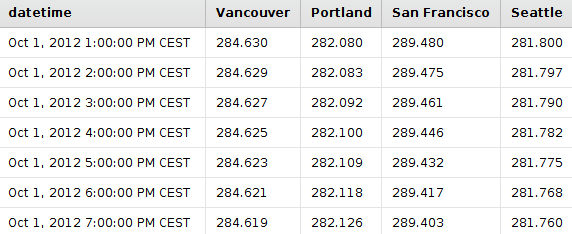
\includegraphics[width=130mm, keepaspectratio]{figures/weather-data-extract.png}
	\caption{Extract from the temperature data set}
	\label{fig:weather-data-extract}
\end{figure}

%---
\section{RapidMiner source}
%---

Concerning the part of the RapidMiner Server, it exposes a process that provides the temperature data from the sample data set. It accepts a parameter determining from which city the user wants to acquire this information. In short, it provides a filtering option by city.

%---
\section{Python source} \label{case-study-python-source}
%---

In this project I demonstrate a proof-of-concept use-case, when the Python data source component reads information from a database and also from an external API service. To be more precise, in the database I store the measured daily minimum and maximum temperature data from 2012 to 2017 in New York. Concerning the the API part, I created a small web application with a REST API that exposes historical highest and lowest temperature values for a given day of the year, also in New York. In the middleware written in Python, I implemented an example business logic which counts on how many days in a month (from October 2012 to November 2017) the measured temperature got close to the all-time records. I have to mention, that the calculation of these historical highest and lowest values is also heuristic. I only took data from January 1959 to September 2012 into account.

I believe, that this is a quite common problem, to have some data in one's storage, but for a better business competence, the usage of external services is also necessary. Hence, this example set-up could serve as an applicable demonstration for further possibilities.
\chapter{Design}

\section{Architecture} \label{arch-design}

The designed architecture of the project can be observed in Figure \ref{fig:arch}. There are three data sources connected to Grafana through an extended version of the official SimpleJSON data source plugin:

\begin{itemize}
	\item RapidMiner Server
	\item JSON backend
	\item Python data source
\end{itemize}

Each data source accesses the data it provides to Grafana in different ways; through an outside service, from a database or from memory.

\begin{figure}[H]
	\centering
	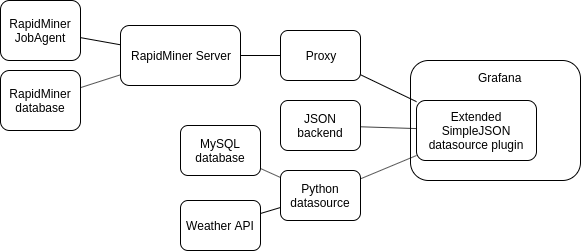
\includegraphics[width=130mm, keepaspectratio]{figures/architecture.png}
	\caption{Architecture diagram}
	\label{fig:arch}
\end{figure}

%---
\section{Components}
%---

In this section, each component's design is presented, focusing on their responsibilities.

%---
\subsection{Extended SimpleJSON datasource plugin} \label{simplejson-design}
%---

Grafana uses data source plugins to connect to different data storage backends. These components usually poll their backends, sending query requests to acquire the recorded information. Each data source plugin exposes a Grafana specific interface, which allows Grafana to communicate with every data source plugin the same way.

% https://github.com/grafana/simple-json-datasource
The SimpleJSON data source is made by the Grafana team and is available on GitHub. \cite{simple-json-datasource}

It has two main purposes. One is to act as an example implementation to make writing custom data source plugins easier for the community. The other is to enable Grafana to read data from services that expose data in JSON format (which is widely popular throughout the industry).

For this thesis project, the latter role seems to be more important, as it is possible to create a tool that receives data from different kind of formats and translates them into JSON. This way, we can send the transformed data to Grafana, which as a result, would be able to display the collected data that originally came from various sources in one place.

Hence, instead of designing a data source plugin for Grafana from scratch, I chose to customize this already available component to dodge many caveats of developing an own plugin for a complex system.

% https://github.com/grafana/simple-json-datasource/blob/master/README.md
The SimpleJSON data source plugin requires its backend to implement the following endpoints:

\begin{itemize}
	\item \emph{/} - This endpoint is used for testing the connection between Grafana and the data backend. If everything is in order on the side of the backend, this endpoint should return a HTTP 200 response.
	\item \emph{/search} - This endpoint is used for finding the available metric options. For example the names of different time series.
	\item \emph{/query} - This endpoint is used to acquire the actual metrics data from the backend.
	\item \emph{/annotations} - This endpoint is used to return objects called annotations that are additional information attached to the metrics data. In the context of this project, we do not use this feature, however, it is needed for the data source plugin to run without errors.
\end{itemize}

In order to introduce additional interactivity capabilities, when integrating the RapidMiner web service, the SimpleJSON data source plugin needs to be extended. Since it is possible for a RapidMiner web service to accept parameters, which can filter the result, it would be useful to be able to acquire these available exposed parameters, so we can make more accurate metric queries with Grafana.

This means that the plugin has to be able to send another type of request to the backend, which in return would respond with the list of the accessible parameters:

\begin{itemize}
	\item \emph{/parameters} - This endpoint is used for acquiring the available query parameters exposed by the backend.
\end{itemize}

During operation, this data source plugin will periodically poll its connected data sources for data, sending HTTP requests to the above described endpoints. The time-interval between the polls depends on the settings in Grafana.

%---
\subsection{Proxy (Gateway)} \label{proxy-design}
%---

The main responsibility of this component is to translate between the RapidMiner web service, which the RapidMiner Server exposes and the SimpleJSON data source plugin. The problem is that RapidMiner Server makes its result available in JSON, but in another format, than the SimpleJSON data source plugin accepts.

To accomplish that this proxy component could communicate with Grafana, it must implement the endpoints required by the SimpleJSON plugin. These were explained in section \ref{simplejson-design} describing the plugin.

So the gateway component should be able to handle HTTP requests from SimpleJSON as well as forwarding them to RapidMiner after the translation. For this reason, it must be a constantly available service.

There are some RapidMiner web service specific considerations which need to be taken into account while designing the gateway component. We have to define the actions made by the proxy towards the RapidMiner Server in an abstract way, in order to properly implement the component.

%---
\subsubsection{Searching the targets}
%---

In order for Grafana to be able to make queries to request data, it needs to know where this data can come from, what is the address of the service that exposes the recorded information. For that, Grafana (and indirectly the SimpleJSON data source plugin) first asks for the available targets of the given data source backend. As it was mentioned in section \ref{simplejson-design}, SimpleJSON uses the \texttt{/search} endpoint for acquiring this information.

In our case, the Proxy component connects to RapidMiner Server, which exposes its data providing processes through web services. Thus, when accepting requests on the \texttt{/search} endpoint the gateway should return with the names of the available RapidMiner web services in a format that the data source plugin accepts. For that, it must send a request to the RapidMiner Server, asking for these names each time, so it is ensured that the information is always up-to-date. This is crucial, as the name of the RapidMiner web service determines the address where the gateway has to send the query requests later.

%---
\subsubsection{Acquiring the parameters}
%---

To enable the customization of the queries, the Proxy's \texttt{/parameters} endpoint should return the parameters exposed by a given web services. This information also falls in the category that should not be cached, as the possession of false knowledge can lead to failed queries that ends up in no data displayed in Grafana.

%---
\subsubsection{Querying the data}
%---
After we have the name of the web service and its available parameters, we can finally request the actual data. To accomplish that,  Grafaba sends a request to the \texttt{/query} endpoint of the Gateway component. Grafana can handle data in two formats: time series, and table (see later in section \ref{impl-qurying}). This means that the Proxy component should be able to convert the acquired data from its backend into one of these formats.

%---
\subsection{JSON backend}
%---
% https://github.com/bergquist/fake-simple-json-datasource
This component is an example backend implementation for the SimpleJSON data source plugin. It serves as a base for creating other backends for the SimpleJSON. It also further expresses the general usability of the plugin. \cite{fake-simple-json-datasource}

As this component can work with the SimpleJSON data source plugin out-of-the-box, I used it during the thesis project mainly for testing purposes. For example to check if the connection is still healthy between the components, or to inspect the specific data formats which are sent to or received from the SimpleJSON plugin.

%---
\subsection{Python data source}
%---

Although Grafana has multiple built-in plugins to communicate with databases, there exists some use-cases, when having a custom component between the data source and the visualization tool is feasible.

With an additional component in the middle, we have extra control over the data, which travels from the data storage backend (in our case, MySQL) to the visualization platform. This means that we do not have to rely solely on the capabilities of the database, which can lead to simpler queries and smaller communication overhead with the database.

Having a custom middleware also makes it possible to implement the business logic in a separate component and only display business-relevant information with the visualization tool.

It also enables us to aggregate information from different backends and provide only one kind of interface towards the visualization which can result in better maintainability. For example in our case, the Weather API component acts as a second backend.

Similarly to the Proxy component, the Python data source also needs to have those endpoints which are required by the SimpleJSON data source plugin, so this part is analogous to that in the Proxy. The effects of invoking them are slightly different than in case of the Gateway, because this Python source uses two components as backends, the 'external' API service and a separate database as described in section \ref{case-study-python-source}. So in order to get the requested data, the Python data source has to turn to both of its backends. This means, that the Python data source has to possess more sophisticated communication capabilities. It needs to be able to handle requests from Grafana, send them back, make connections to the database and query its contents and to send requests to the 'external' API service and accept the results from it.

%---
\subsection{Weather API}
%---

As it was already described in section \ref{case-study-python-source} describing the sample use-case, I implemented a simple service, that can return the all-time (calculated in a heuristic way, as it was already mentioned) maximum and minimum temperatures measured in New York for a given day of the year.

This component represents the previously mentioned external service. Its responsibility is to expose a service that can be utilized by other softwares in order to acquire additional business-relevant information.

% https://openweathermap.org/api
% https://developer.accuweather.com/

It is worth to mention, that there are already several publicly available APIs that can be used to retrieve weather related data. For example, the API services of OpenWeather\cite{openweather} or AccuWeather\cite{accuweather}. However, these services are usually not free or only offer a free trial version, which lasts just a couple of days long. This is why I decided to make an own API service that can be used during the whole time of preparing the thesis project.

%---
\subsection{MySQL database}
%---

In section \ref{case-study-python-source}, it was stated, that one of the backends used by the Python data source is a separate database. This database stores the data of the measured daily maximum and minimum temperatures in New York throughout a couple of years.

%\begin{itemize}
%	\item why do we need a gateway
%	\item how can we access data from RapidMiner WebService
%	\item why is it good to have a python compoment between Grafana and MySQL
%	\begin{itemize}
%		\item we can customize it better, what we see from the database
%		\item can implement business logic, only see business-relevant projections, granularity of the data
%		\item can aggregate data from different backends
%		\item can aggregate data with outsider APIs (POC implementation for this use-case)
%	\end{itemize}
%\end{itemize}


%\begin{itemize}
%	\item Grafana
%	\item proxy/gateway
%	\item python-datasource
%	\begin{itemize}
%		\item python-datasource
%		\item mysql
%		\item weather-api
%	\end{itemize}
%	\item RapidMiner stack
%	\begin{itemize}
%		\item rapidminer-server
%		\item job-agent
%		\item database
%	\end{itemize}
%	\item Grafana datasource plugin (extended API - parameters)
%	\begin{itemize}
%		\item extended API for asking for available parameters
%		\item extended GUI, that dynamically lists available parameters (specify SOURCE!!!!!!!)
%	\end{itemize}
%	\item Grafana extended panel plugin
%\end{itemize}
\chapter{Implementation}

In this chapter, the previously described components are explained in further details, focusing on how they are implemented, what technologies were used and in addition, some extra fine tunes are presented, which demonstrate the extendability of the open source Grafana.

The source code for the thesis project is available and can be viewed in my GitHub repository.\cite{thesis-repo}

\section{Architecture}

%---
\subsection{Docker}
%---
% https://www.docker.com/resources/what-container

Throughout this project, I run the different components using Docker containers. For this reason, it seems appropriate to briefly introduce this technology.

A container is a standard unit of software that packages up code and all its dependencies so the application runs quickly and reliably from one computing environment to another. A Docker container image is a lightweight, standalone, executable package of software that includes everything needed to run an application: code, runtime, system tools, system libraries and settings.

Container images become containers at runtime and in the case of Docker containers - images become containers when they run on Docker Engine. Available for both Linux and Windows-based applications, containerized software will always run the same, regardless of the infrastructure. Containers isolate software from its environment and ensure that it works uniformly despite differences for instance between development and staging.\cite{docker}


\subsection{Docker Compose}

In order to be able to set up an architecture as the one described in section \ref{arch-design}, I used Docker Compose.

% https://docs.docker.com/compose/

Docker Compose is a tool for defining and running multi-container Docker applications. With Compose, we can use a YAML file to configure application’s services. Then, with a single command, we can create and start all the services from the configuration.\cite{docker-compose}

The \texttt{docker-compose.yml} file for the project can be found in the GitHub repository of the thesis project. It defines all the necessary components with the appropriate configuration.

\vspace{0.5cm}
\begin{minipage}{\linewidth}
	\begin{lstlisting}[language=docker-compose-proxy, caption={Extract of the \texttt{docker-compose.yml}}, label={lst:proxy-docker-compose}]]	
	  proxy:
	    build: ./proxy
	    ports:
	    - 5000:5000
	    restart: always
	    volumes: 
	    - "./proxy/proxy.py:/code/proxy.py"
	\end{lstlisting}
\end{minipage}

\section{Proxy (Gateway)} \label{proxy-impl}

It was established in the design section \ref{proxy-design}, that the main responsibility of the Gateway component is to translate between the JSON data formats used by the RapidMiner Server and the Grafana SimpleJSON data source plugin.

For this task, I had two possibilities. One is to use a tool, which defines the transformation in a declarative way. For example, I could use XLST, which is able to convert a JSON format into another \cite{xslt}. The other option was to implement an own algorithm which handles the transformation of the data format. I chose the latter alternative as the structure of the data was not exceptionally complex, thus it was quite simple to implement a function for this job . The other reason was that this way, I did not have to integrate another tool and call it every time to transform a simple JSON object, which in general reduced the number of possible sources for errors.

% https://www.xml.com/articles/2017/02/14/why-you-should-be-using-xslt-30/

As it was described in section \ref{proxy-design}, the Gateway component must be able to handle requests from Grafana, as well as be able to forward these requests to the RapidMiner Server after the format translation. 

% https://www.palletsprojects.com/p/flask/
% https://realpython.com/python-requests/
For this task, I implemented the Gateway in Python using the \texttt{flask}\cite{flask} and the \texttt{requests}\cite{requests} packages and ran it in a Docker container. Flask is a lightweight web application framework library that enables quick and simple development. Requests can be thought of as the de facto standard for making HTTP requests in Python. It abstracts the complexities of making requests behind a simple API.

%---
\subsection{Endpoints}
%---

As it was explained in section \ref{proxy-design}, the Gateway component has to expose the endpoints that are required by the SimpleJSON data source plugin.

With the \texttt{requests} package, it is quite convenient to implement these endpoints, since we only have to declare a decorated function for each endpoint, as it is shown in the code snippet \ref{lst:proxy-test-conn}.

\vspace{0.5cm}
\begin{minipage}{\linewidth}
\begin{lstlisting}[language=Python, caption={Test the connection to the server}, label={lst:proxy-test-conn}]]
	@app.route('/')
	def check_connection():
	  response = requests.get(server_host)
	    if response.status_code == 200:
	      return 'Server connection OK'
	  return "Server connection error"
\end{lstlisting}
\end{minipage}
%---
\subsubsection{Searching the targets}
%---

To be able to get the names of the available RapidMiner web services, the Gateway component should use the \texttt{/api/rest/service/list} endpoint of the RapidMiner Server. This endpoint returns the names and parameters of the web services in JSON format. The Gateway extracts the names of the services transforms this data into a format that SimpleJSON can understand.

The endpoint is implemented as displayed in the following \ref{lst:proxy-search} code snippet. 

\begin{minipage}{\linewidth}
\begin{lstlisting}[language=Python, caption={Get the names of the web services}, label={lst:proxy-search}]]
@app.route('/search', methods=['POST'])
def search():
  response = requests.get(server_host + '/api/rest/service/list',
                          auth=('admin', 'changeit'))
  webservices_json_list = json.loads(response.text)
  webservice_names = []
  for webservice in webservices_json_list:
    webservice_names.append(webservice['name'])
  return json.dumps(webservice_names)
\end{lstlisting}
\end{minipage}
%---
\subsubsection{Acquiring the parameters}
%---

To get the available parameters of the exposed web services, the Gateway component uses the same endpoint of the RapidMiner Server (\texttt{/api/rest/service/list}), as for searching the targets.

The reason for that these two features are separated, even though they use the same endpoint, is that concerning the Gateway, the functionality of exposing the available targets is required by the SimpleJSON by default while querying the parameters is an extra feature. This means that SimpleJSON expects a specific data format, which only includes the names of the targets. Thus returning the parameters additionally with the targets would break the compatibility between the Gateway component and the SimpleJSON data source plugin.

Acquiring the parameters is implemented the following way, as in the code snippet \ref{lst:proxy-params}.

\begin{minipage}{\linewidth}
	\begin{lstlisting}[language=Python, caption={Get the parameters for a given web service}, label={lst:proxy-params}]]
	@app.route('/parameters', methods=['GET'])
	def parameters():
	  if request.args:
	    args = request.args
	    webserviceName = args.get('webserviceName')
	    if webserviceName == None:
	      raise ValueError('No value provided for "webserviceName"')
	    # get the list of webservices and get the parameters of the one with the name provided in the query
	    response = requests.get(server_host + '/api/rest/service/list',
	    auth=('admin', 'changeit'))
	    webservices_json_list = json.loads(response.text)
	    webservice_params = []
	    for webservice in webservices_json_list:
	      if webservice['name'] == webserviceName:
	        webservice_params = webservice['parameters']
	        break
	    return json.dumps(webservice_params)
	  return 'Please provide a query parameter in the URL'
	\end{lstlisting}
\end{minipage}

%---
\subsubsection{Querying the data}\label{impl-qurying}
%---
When Grafana sends a request to the Gateway component, it specifies the data format, in which it excepts to receive the results. This can be a time series format or a table format which can be seen in the code snippets below.

\begin{minipage}[b]{0.45\linewidth}
	\centering
	\begin{lstlisting}[language=Python, frame=single, numbers=left, mathescape,%
	caption={Time series format}, label=lst:timeseries-format]
	[
	 {
	    "target":"weather_retrieve_process?city=Vancouver",
	    "datapoints":[
	      [284.63, 1573882025382],
	      [284.629, 1573885625382],
	      [284.627, 1573889225382],
	      [284.625, 1573892890284],
	      [284.623, 1573896490284],
	      [284.621, 1575746856319],
	      [284.619, 1575750456319],
	      [284.617, 1575754056319]
	    ]
	 }
	]
	\end{lstlisting}
\end{minipage}
\hspace{0.5cm}
\begin{minipage}[b]{0.45\linewidth}
	\centering
	\begin{lstlisting}[language=Python, frame=single, mathescape,%
	caption={Table format}, label=lst:table-format]
	[
	 {
	   "columns":[
	     {"text":"Month","type":"string"},
	     {"text":"Maxs","type":"number"}
	   ],
	   "rows":[
	     ['2012 October', 1],
	     ['2012 November', 1],
	     ['2012 December', 0],
	     ['2013 January', 0]
	   ],
	   "type":"table"
	 }
	]
	\end{lstlisting}
\end{minipage}

The time series response format contains the target name, which in this case is the name of the RapidMiner web service with an additional parameter attached to it and the data points. The first value in a data point is the actual value, the second is the timestamp in UNIX Epoch time in milliseconds.

The table format describes the name and the type of each column in the \texttt{columns} array. The actual data is in the \texttt{rows} array, every row is defined with a list of values in an order that is correspondent to that of the columns.

%---
\section{Python data source}
%---

As it was mentioned in section \ref{case-study-python-source} and section \ref{proxy-design}, the Python data source communicates with a database and a separate API service in order to prepare the requested data for Grafana.

The Python data source is also connected to Grafana, so it needs to expose the endpoints that are needed by the SimpleJSON data source plugin (discussed in section \ref{simplejson-design}), which are implemented similarly as in the Gateway.

The differing ability of the Python data source compared to the Gateway  component is that it can connect to a MySQL database and an external API to get the requested data by Grafana. To be able to implement these features, I used the \texttt{requests} and the \texttt{mysql.connector} packages along with the \texttt{flask} library, which is needed to be able to send HTTP requests (as in the case of the Gateway component).

% # https://pynative.com/python-mysql-select-query-to-fetch-data/

Reading the data from the MySQL database is implemented as the following pseudo code shows (\ref{lst:mysql-conn}).

\vspace{0.5cm}
\begin{minipage}[b]{\linewidth}
	\centering
	\begin{lstlisting}[language=Python, frame=single, mathescape,%
	caption={Reading data from MySQL}, label=lst:mysql-conn]
	def read_data_from_db():
	  try:
	    connection = mysql.connector.connect(
	      <credentials>
	    )
	    sql_select_records_query = "SELECT * FROM newyork"
	    cursor = connection.cursor()
	    cursor.execute(sql_select_records_query)
	    records = cursor.fetchall()
	    data = []
	    for row in records:
	      record = {
	        <parse data from a record>
	      }
	      data.append(record)
	    return data
	  except Error as error:
	    print("Error reading data from MySQL ", error)
	  finally:
	    <close the connection to the database>
	\end{lstlisting}
\end{minipage}

Getting the recorded information from the 'external' Weather API is much simpler thanks to the level of abstraction the \texttt{requests} package provides. (\ref{lst:weather-conn})

\vspace{0.5cm}
\begin{minipage}[b]{\linewidth}
	\centering
	\begin{lstlisting}[language=Python, frame=single, mathescape,%
	caption={Reading data from the Weather API}, label=lst:weather-conn]
	def get_all_time_records():
	  response = requests.get(weather_api_host + '/all')
	  json_data = json.loads(response.text)
	  return json_data
	\end{lstlisting}
\end{minipage}

After the Python data source possesses the data both from the MySQL database and the Weather API, it aggregates the collected information (\texttt{create\char`_table\char`_data()} function) according to the sample business-logic already discussed in section \ref{case-study-python-source} and then exposes it on its \texttt{/query} endpoint. (\ref{lst:python-query})

\begin{minipage}[b]{\linewidth}
	\centering
	\begin{lstlisting}[language=Python, frame=single, mathescape,%
	caption={Exposing the prepared data}, label=lst:python-query]
	@app.route('/query', methods=['POST'])
	def query():
	  table_data = create_table_data()
	  return json.dumps(table_data)
	\end{lstlisting}
\end{minipage}

%---
\section{Additional features}
%---

After the integration of the two data sources, I implemented some additional features in Grafana to increase its interactivity capabilities. These are mainly developments in the graphical interface, thus they do not affect the already presented architectural model.

%---
\subsection{Customized Grafana Query Editor GUI}
%---

As it was already discussed in section \ref{query-editor}, the Query Editor determines what data Grafana requests from its data sources, hence, what data will be visualized on the panel. 

With the usage of the extra \texttt{/parameters} endpoint of the Gateway component, I implemented the dynamic listing of available parameters for a web service in the Query Editor of the extended SimpleJSON data source plugin.

This means that the user does not have to be familiar with the exact name or amount of the exposed parameters for a web service. When he or she chooses a target to query, Grafana asks the data source to get this information. An example of this dynamic parameter listing can be seen in Figure \ref{fig:dynamic-parameters}. There we have a RapidMiner web service called \texttt{Predicitve\char`_Maintanence\char`_web\char`_service\char`_with\char`_parameters} with two available parameters called \texttt{machineID} and \texttt{sensor1}.

\begin{figure}[h]
	\centering
	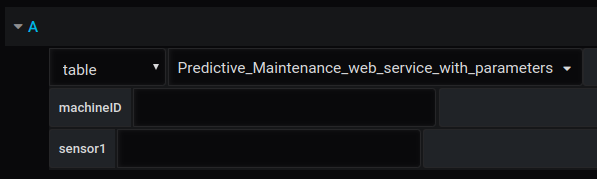
\includegraphics[width=130mm, keepaspectratio]{figures/dynamic-parameters.png}
	\caption{Dynamic listing of available parameters}
	\label{fig:dynamic-parameters}
\end{figure}

%---
\subsection{Dynamic bar chart in Grafana} \label{dynamic-barchart}
%---
% https://github.com/CorpGlory/grafana-graph-panel

In section \ref{grafana-time-range-controls}, it was already discussed, that it is possible to change the time interval of the whole Dashboard by selecting a time range on a Graph Panel.

% https://grafana.com/docs/grafana/latest/features/panels/graph/
The Graph Panel offers other display possibilities as well apart from the graph diagram. It can visualize time series data with bar-charts and histograms \cite{graph-panel}. I focused on the bar-chart format, which groups the data by series and not time, so with this type of diagram, we can display aggregated information about the series. For example the total value, the average, the maximum or the count of the data points.

However, I noticed, that when I change the time range of the Dashboard, these basic statistical indices do not get refreshed based on the new time interval. They keep their original values that were calculated for the whole time series when Grafana received the information from one of its data sources. This phenomenon can be quite misleading in cases when we have multiple Graph Panels with the same querying settings, but with different visualization modes.

To solve this issue, as a part of my thesis project, I successfully extended the built-in Graph Panel, so it calculates the aggregated values only from the data points that are in the time interval of the dashboard. This feature enables a more interactive and valuable insight of the visualized data.

To accomplish this, I used the source code of the built-in Graph Panel configured with the \texttt{webpack} module bundler which enabled the simple integration of this customized panel as a separate plugin for Grafana. \cite{graph-panel-webpack}

%---
\section{Grafana Dashboard} \label{final-dashboard}
%---

As a final, easy to demonstrate result of the integration task of this project, I created a Dashboard in Grafana to display the collected data from various sources that can be seen in Figure \ref{fig:dashboard-final}. As it was already expressed in chapter \ref{case-study}, I used a sample data set containing information about weather in different cities in order to be able to visualize the results of the created architecture.

\begin{figure}[h]
	\centering
	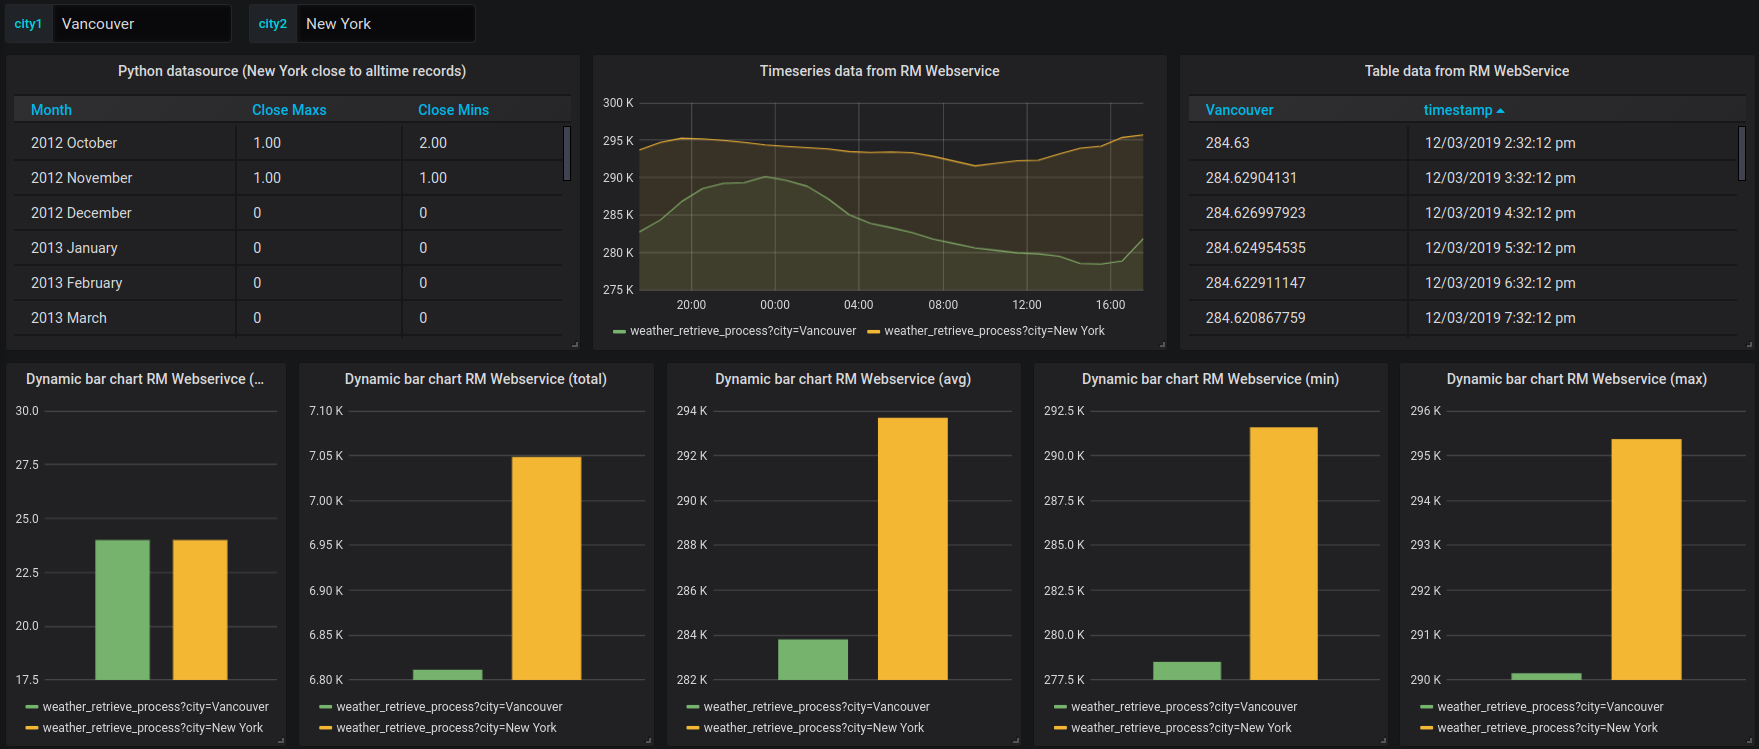
\includegraphics[width=\linewidth, keepaspectratio]{figures/final-dashboard.png}
	\caption{Dashboard showing the results}
	\label{fig:dashboard-final}
\end{figure}

The Graph Panel in the middle shows the same two time series data as the five bar-chart diagrams that display some basic statistical indices in a time-dependent manner as discussed before in section \ref{dynamic-barchart} introducing the dynamic bar-chart.

All the visualized data on this Dashboard comes from the RapidMiner Server component through exposed web services, expect for the table in the top-left corner, which shows recorded information originating from the Python data source unit.

On the top of the Dashboard, two templating variables can be seen, which determine the two cities that we use to filter the displayed data.

\chapter{Evaluation}

In this chapter, I present the evaluation of the implemented Gateway component, introducing its advantages and disadvantages.

%---
\section{Advantages}
%---

The Gateway component I created, successfully suits the declared requirements discussed in section \ref{goals} and \ref{proxy-design}.

It implements the necessary interfaces in order to be able to communicate with Grafana (specifically, with the SimpleJSON data source plugin). It can also send requests to its backend storage, which is a RapidMiner Server exposing multiple web services.

It conforms to the expectations of having the capabilities to transform between the data format that the RapidMiner Server uses to provide its results and the format that the SimpleJSON data source plugin requires so it can parse the requested data in order for it to be visualized in Grafana.

Furthermore, the Gateway component introduced a new feature to the built-in SimpleJSON. It enabled the querying of  the available parameters for each web service, which made it possible to dynamically list them for the user, who now does not have to be familiar with the details of customizing the queries. This ability enforces the many interactivity features of Grafana.

Regarding the effectiveness of this component, there is also an operations related convenience that needs to be mentioned among its advantages. The created Gateway runs in a Docker container, which enables the simple portability of this tool, enhancing it usability in various types of environments.

%---
\section{Disadvantages} \label{proxy-cons}
%---
% production ready webserver
% use of decarative data tranformation in case of more complex data structure in the future
% in case of static processes, which result do not change over time, or just daily, cache the results, this needs improvement, more meta information from the RM side too ->>> querying the possible parameter values

% to fill out the city variable, one has to know, which cities are in the dataset, --> enable querying meta information about the data set, e.g. the name of the columns

% security credentials are hard-coded, improvements on this side, at least read them from an environment variable that is included in the container on startup

Despite that the Proxy component conforms to all of the expressed requirements, there are also some disadvantages that present room for further improvements.

First of all, the way it is currently realized is that it runs on a \texttt{flask} development server that enables quick progress during the implementation phase, however, it does not provide favorable performance in a production grade environment.

Concerning the data format transformation, it was discussed in section \ref{proxy-impl} why I did not choose an existing tool that enables defining JSON transformations in a declarative way. Yet, in order to prepare for more complex data structures in the future, it would be profitable to integrate such a tool instead of further extending my own algorithm.

Another downside of the current implementation is that it does not provide any information about the possible values of the available parameters. For example in the case of the Dashboard that was mentioned in section \ref{final-dashboard}, the user does not know which cities can write into the text box of the variable without further knowledge about the data set. Of course, in order for this functionality to work, the backend storage would have to support it too, but nonetheless, the Gateway component could have this feature.

There is also a performance issue regarding the Gateway component which does not reside on code level, but rather in the design. There are use-cases, when the exposed processes are not time-dependent or change their results over longer periods of time, for example every day or week. Querying these processes too frequently can cause a significant unnecessary overhead for the system. Some kind of caching method would probably solve this problem, for example if the Proxy component tracked the incoming requests by the name of the web service and the attached parameters. Additionally, the backend storage would have to expose some meta information about processes of such kind, providing the usual time interval for each process after which the results are probably different as those of the previous queries.

I have to mention some security concerns too about the current realization of the Gateway component. In order to be able to query the results of the web services, one must posses the correct credentials to invoke these endpoints on the RapidMiner Server. At the moment, these credentials are hard-coded into the Proxy component, which presents a serious security vulnerability. A possible solution for this problem would be reading these sensitive information from environment variables, which are set on container startup.

%---
\section{Focus on time series}
%---

Grafana mainly concentrates on the visualization of time-dependent data. This can be deduced from the fact that the majority of the data sources, which Grafana supports, are storing data time series data or data with a timestamp attribute. However, despite the heavy time series focus, it is capable of working with other data formats as well.

The created Gateway component is able to handle the time series format and also the table format, which is used to display other formats of data in Grafana, for example, recorded information from a relational database.



\chapter{Future work}

In this chapter, some possibilities for future development are discussed concerning the implemented components of this thesis project.

First of all, it must be mentioned that during this thesis project, writing optimal code for the various implementations was not priority, as the main focus of this work was the integration of different tools. Hence, a feasible enhancement could be to rewrite the custom parts and components concentrating on the performance.

\section{Gateway}

One possible development of the Gateway component could be to integrate it with the SimpleJSON data source plugin in order to create one tool to connect RapidMiner Server with Grafana. This would introduce several advantages compared to the current architectural setup.

Merging the Gateway component with SimpleJSON would mean, that the data format translation between these units could happen directly in Grafana. Thus, the communication overhead of the system could be reduced, as there would not be an extra component on the path of the data to be collected.


% https://grafana.com/grafana/plugins?orderBy=weight&direction=asc

Another advantage of having one component instead of two is in regard of packaging and distribution. As it was already stated, Grafana is an open source project, meaning it heavily relies on the contribution of the community. Grafana allows the development of custom Data Sources - and also Panels - that can be published on the Grafana plugin marketplace. With an integrated component it would be easier to accomplish to have a publicly available data source plugin specifically for RapidMiner Server.

Further alternatives for improving the Proxy component can be the amendment of its disadvantages, which are discussed in section \ref{proxy-cons}.

%---
\section{Dynamic Graph Panel}
%---

Concerning the time-dependent bar-chart visualization mode in the modified Graph Panel, there are also some alternatives to improve it in the future.

Currently, the extended Graph Panel displays the series defined in its Query Editor according to the time interval of the Dashboard only, when its selected visualization mode is graph-diagram (Time mode) or bar-chart (Series mode). But there exists a third mode, called Histogram. The possible improvement of this Panel could be to modifiy the Histogram to be time-dependent too.

Another potential enhancement would be to implement a feature that enables the possibility to switch between the time-dependent mode and the original static mode of calculating the basic statistical indices of the time series data. This would lead to the result that only one Graph Panel type would be needed, as right now, the user can choose between to original Graph Panel and the extended one, however, looking at their capabilities in general, they offer the same features.
\chapter{Related works}

grafana data source plugins -> they integrate different kind of backends with grafana

interactive-piechart-panel (github/eastcirclek)
see notebook

\chapter{Summary}

Nowadays, organizations must handle the challenging task of managing data coming from all kinds of sources with varying features including the data format, the frequency of new information records and the peculiarity of the different technologies they are built with. There are plenty of reasons why merging the data from various sources is so profitable, for example it enables the visualization of the collected data in one place in order to provide a clean, understandable way of overseeing the ongoing processes and results in a company.

In this thesis, I first 



\begin{itemize}
	\item introduce datasorces, features
	\item research on Grafana
	\item interactivty
	\item integration of RM Server with Grafana
	\item Python data source between MySQL and Grafana
	\item additional GUI features to increase interactivity features
	\item discussing possibilities for further improvements, pros/cons
	\item research on related works
\end{itemize}




% Acknowledgements
%~~~~~~~~~~~~~~~~~~~~~~~~~~~~~~~~~~~~~~~~~~~~~~~~~~~~~~~~~~~~~~~~~~~~~~~~~~~~~~~~~~~~~~
%----------------------------------------------------------------------------
\chapter*{\koszonetnyilvanitas}\addcontentsline{toc}{chapter}{\koszonetnyilvanitas}
%----------------------------------------------------------------------------

I would like to thank all the people, who helped me during the semester to prepare this thesis, without being exhaustive. My advisor, Dr. Zoltán Szatmári, who guided me through the work and gave countless professional advice in order to ensure the success of the project. I thank my colleagues at RapidMiner for providing me with many practical suggestions. I would also like to thank my roommates, Balázs Prehoda and Kornél Tamás, who constantly motivated me with their hard work and commitment concerning their own thesis projects. Finally, I would like to thank Eszter Zsubori and Peter Orova for helping me revise the stylistics of this work.


% List of Figures, Tables
%~~~~~~~~~~~~~~~~~~~~~~~~~~~~~~~~~~~~~~~~~~~~~~~~~~~~~~~~~~~~~~~~~~~~~~~~~~~~~~~~~~~~~~
%\listoffigures\addcontentsline{toc}{chapter}{\listfigurename}
%\listoftables\addcontentsline{toc}{chapter}{\listtablename}


% Bibliography
%~~~~~~~~~~~~~~~~~~~~~~~~~~~~~~~~~~~~~~~~~~~~~~~~~~~~~~~~~~~~~~~~~~~~~~~~~~~~~~~~~~~~~~
\addcontentsline{toc}{chapter}{\bibname}
\bibliography{bib/mybib}


% Appendix
%~~~~~~~~~~~~~~~~~~~~~~~~~~~~~~~~~~~~~~~~~~~~~~~~~~~~~~~~~~~~~~~~~~~~~~~~~~~~~~~~~~~~~~
% %----------------------------------------------------------------------------
\appendix
%----------------------------------------------------------------------------
\chapter*{\fuggelek}\addcontentsline{toc}{chapter}{\fuggelek}
\setcounter{chapter}{\appendixnumber}
%\setcounter{equation}{0} % a fofejezet-szamlalo az angol ABC 6. betuje (F) lesz
\numberwithin{equation}{section}
\numberwithin{figure}{section}
\numberwithin{lstlisting}{section}
%\numberwithin{tabular}{section}

%----------------------------------------------------------------------------
\section{A TeXstudio felülete}
%----------------------------------------------------------------------------
\begin{figure}[!ht]
\centering
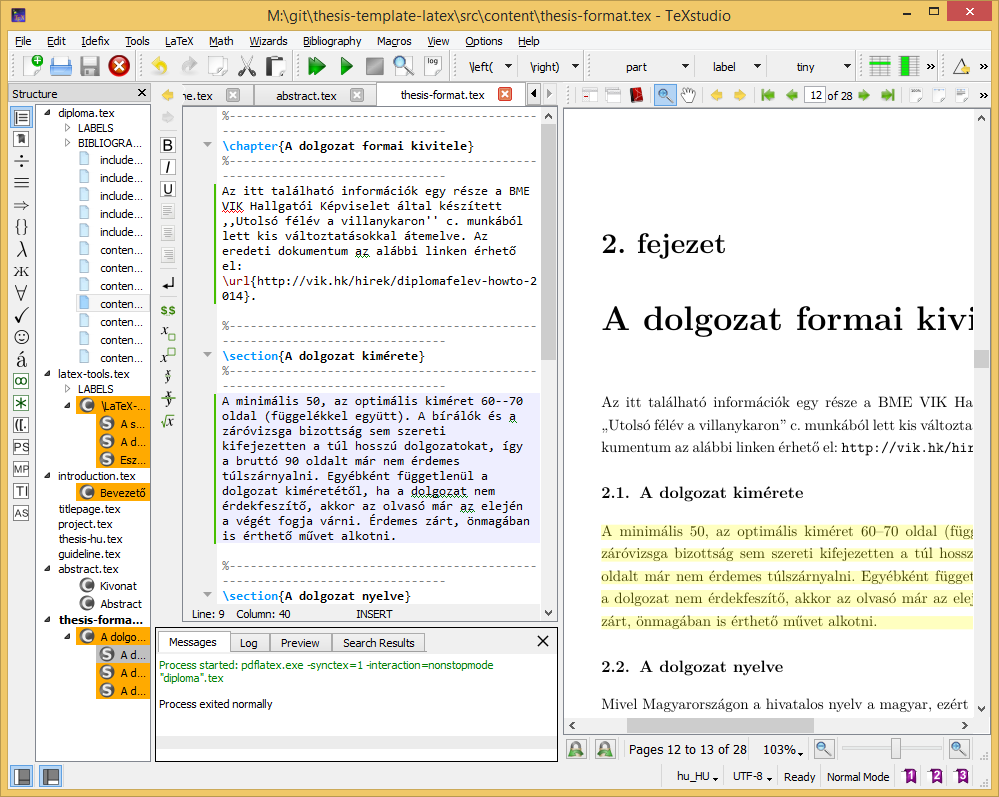
\includegraphics[width=150mm, keepaspectratio]{figures/TeXstudio.png}
\caption{A TeXstudio \LaTeX-szerkesztő.} 
\end{figure}

%----------------------------------------------------------------------------
\clearpage\section{Válasz az ,,Élet, a világmindenség, meg minden'' kérdésére}
%----------------------------------------------------------------------------
A Pitagorasz-tételből levezetve
\begin{align}
c^2=a^2+b^2=42.
\end{align}
A Faraday-indukciós törvényből levezetve
\begin{align}
\rot E=-\frac{dB}{dt}\hspace{1cm}\longrightarrow \hspace{1cm}
U_i=\oint\limits_\mathbf{L}{\mathbf{E}\mathbf{dl}}=-\frac{d}{dt}\int\limits_A{\mathbf{B}\mathbf{da}}=42.
\end{align}


%\label{page:last}
\end{document}
